\label{simulation}
\section{Simulation}

\begin{frame}{Simulation}
    \begin{center}
        \Large \textbf{A computational approach}
    \end{center}
    \centering
    \begin{itemize}
        \item<1-> \alert{Simulate} the evolution of the system by reproducing the steps of the Ehrenfest model
        \item <2-> Run the simulation for a \alert{large number of time steps}
        \item<3-> \alert{Estimate} the asymptotic quantities by sampling them
    \end{itemize}
\end{frame}

\begin{frame}{Simulation}
  \Large
  \centering
  \textsc{Results: Limiting Distribution}
  
\end{frame}

% \begin{frame}{Simulation}
%     \Large Example: limiting distribution
%     \normalsize
%     \begin{itemize}
%         \item $N = 100$
%         \item Initial condition: $X_0 = N$
%         \item Plots for the sample visit frequencies $t = 0$, $t = 100$, $t = 1000$ and the convergence
%     \end{itemize}
    
% \end{frame}

\begin{frame}
    \begin{figure}
        \begin{subfigure}{.49\textwidth}
            \centering
            \includegraphics[width=\linewidth]{pictures/evolution_0.pdf}
            % \caption{$t = 0$}
          \end{subfigure}
          \begin{subfigure}{.49\textwidth}
            \centering
            \includegraphics[width=\linewidth]{pictures/evolution_1.pdf}
            % \caption{$t = 100$}
          \end{subfigure}\\
          \begin{subfigure}{0.49\textwidth}
            \centering
            \includegraphics[width=\linewidth]{pictures/evolution_2.pdf}
            % \caption{$t = 1000$}
          \end{subfigure}%
          \begin{subfigure}{0.49\textwidth}
            \centering
            \includegraphics[width=\linewidth]{pictures/evolution_3.pdf}
            % \caption{At convergence}
        \end{subfigure}\\
        \begin{center}
          \begin{subfigure}{0.4\textwidth}
            \centering
            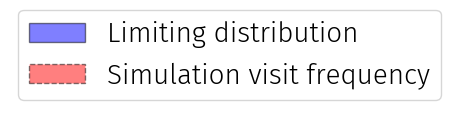
\includegraphics[width=\linewidth]{pictures/legend.png}
            % \caption{At convergence}
          \end{subfigure}\\
        \end{center}
        \end{figure}
\end{frame}

% \begin{frame}{Simulation}
%     \Large
%     Example: mean recurrence time
%     \normalsize
%     \begin{itemize}
%       \item use a fixed number of time steps $T = 10^7$
%       \item good estimates only for some value of $N$
%       \item plots for $N = 10$, $N = 15$, $N = 20$, $N = 30$
%     \end{itemize}
% \end{frame}

\begin{frame}{Simulation}
  \centering \Large
  \textsc{Results: Mean Recurrence Time}
\end{frame}

\begin{frame}
  \begin{figure}
      \begin{subfigure}{.49\textwidth}
          \centering
          \includegraphics[width=\linewidth]{pictures/recurrence_0.pdf}
          % \caption{$t = 0$}
        \end{subfigure}
        \begin{subfigure}{.49\textwidth}
          \centering
          \includegraphics[width=\linewidth]{pictures/recurrence_1.pdf}
          % \caption{$t = 100$}
        \end{subfigure}\\
        \begin{subfigure}{0.49\textwidth}
          \centering
          \includegraphics[width=\linewidth]{pictures/recurrence_2.pdf}
          % \caption{$t = 1000$}
        \end{subfigure}%
        \begin{subfigure}{0.49\textwidth}
          \centering
          \includegraphics[width=\linewidth]{pictures/recurrence_3.pdf}
          % \caption{At convergence}
      \end{subfigure}\\
      \begin{center}
        \begin{subfigure}{0.26\textwidth}
          \centering
          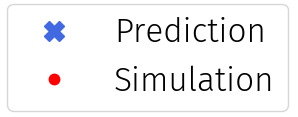
\includegraphics[width=0.9\linewidth]{pictures/legend_2.png}
          % \caption{At convergence}
        \end{subfigure}\\
      \end{center}
      \end{figure}
\end{frame}